\chapter{Extended Abstract}

% ###
% Beginning of the extended abstract. We will use english in this chapter.
\selectlanguage{english}
% ###

{
\newtheorem*{abstract}{Abstract}

\begin{abstract}
    Efficient construction of the \emph{suffix array} (\sa) is a still ongoing research area.
    We introduce SACABench, a benchmark system for comparing the runtime
    and memory consumption of \emph{suffix array construction algorithms} (SACAs).
    Along with this framework we include the reference implementations for many SACAs,
    parallel and sequential, as well as our own implementations.
    Although they are slower than their reference implementations in most cases,
    they can be helpful to understand the algorithms because they are written in modern C++.
    In our evaluation we compare the performance of these algorithms
    in single-threaded and multi-threaded environments.
\end{abstract}
}

\section{Introduction}

The \currentauthor{Marvin Böcker} \emph{suffix array} (\emph{\sa}) is a widely known text index,
which can be used for various string operations,
like full-text search~\cite{makinen} and construction of the Burrows-Wheeler Transform (BWT)~\cite{BWT}.
It is a permutation of all indices $1 \dots n$ of a text of length $n$ such
that the $i$th suffix of the text \inputtext has lexicographic rank $\sa[i]$.

While the efficient construction is still an active research area,
divsufsort~\cite{saca:5,saca:5:repo} is the empirically fastest
suffix array construction algorithm (SACA) since 2008,
even though it has a theoretical complexity of $\mathcal O (n \log n)$,
while there are several $\mathcal O(n)$ algorithms (for example SAIS\cite{saca:6} and DC3~\cite{saca:9}) available.

For the last year we (re-)implemented eleven SACAs~\cite{saca:3,saca:11,saca:5,saca:9,saca:1,saca:8,saca:4,saca:7,saca:10,saca:6,saca:2}
in modern C++ in order to create faster and more memory efficient implementations.
In the process we created a sophisticated benchmark framework for SACAs, \emph{\sacabench}~\cite{sacabench:github}.
In this paper we introduce our framework and highlight its features,
as well as document some of the optimiziation strategies we used to implement the SACAs.
In the end we give an overview and performance comparison of the popular SACAs,
as well as the current landshape of parallel SACAs.

\section{Benchmark Tool}

\sacabench is a CMake/C++14 project which contains many different SACAs.
There are both sequential and parallel algorithms included
and we also include the reference implementations for all of the algorithms, if one exists.
It is also possible to include a new or another existing SACA with \sacabench
\footnote{For instructions on how to do this, please consider our README in the GitHub Repository~\cite{sacabench:github}}.
You are able to run a single, a subset of, or all of the algorithms, depending on your needs.
Time and memory consumption is automatically measured and can be output as JSON.
We also include tools to convert the JSON-format to graphs for a visual comparison of the algorithms.

This is the most important aspect of our framework:
the possibility to easily run many SACAs on the same input text on the same hardware
in order to measure and compare them fairly.

\subsection{Running a single algorithm}

\begin{figure}[!ht]
    \centering
    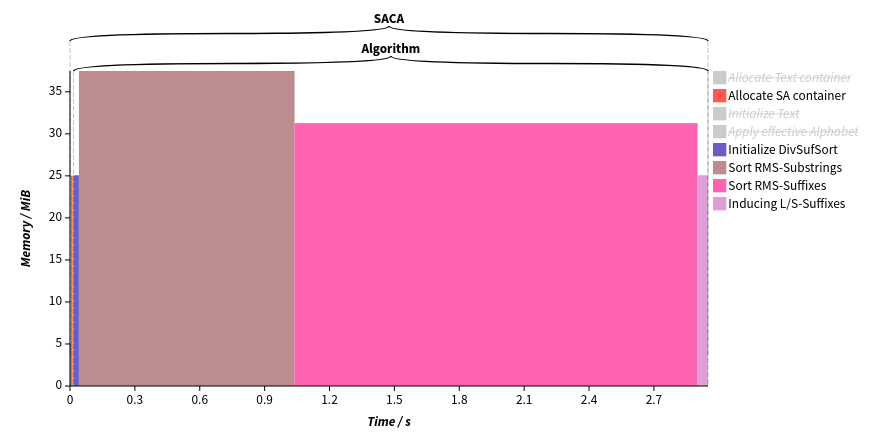
\includegraphics[width=\textwidth]{kapitel/1_extended_abstract/tudostat_example.png}
    \caption{Example of runtime and memory consumption of the phases of DivSufSort, measured by \sacabench and visualized on the tudostat website~\cite{tudostat}.}
    \label{ea:phases}
\end{figure}

You can evaluate a single algorithm with the command \termfont{sacabench construct} followed by the desired SACA and a path to an input file.
To get a list of all available Algorithms, you can execute the command \termfont{sacabench list}.
This will output the names for all available SACAs.

While the algorithm is running, its memory consumption is measured via the tudostat library~\cite{tudostat}.
You can also enable checking of the resulting suffix array with a fast suffix array checker~\cite{saca:11} by
using the \termfont{-c} or a parrallel version with the \termfont{-q} flag.
To generate a JSON file containing detailed information about the run of the selected Algorithm separated into SACA-specific phases,
the flag \termfont{-b} needs to be added to the command, followed by a destination path to which the report will be saved to.
To override an existing file at the destination path, the option \termfont{-f} can be used.
This file can be converted to a plot on the tudostat website~\cite{tudostat} (see Figure \ref{ea:phases} as an example).
If you add the flag \termfont{-{}-rplot}, a plot will be generated automatically after the SACA executed by using an R-script.
Additionally there is an alternative version of plots, which are generated using LaTex.
This can be done by adding the flag \termfont{-{}-latexplot}.

Multiple other flags and options allow to customize the way, the SACA is executed.
For example, it is possible to use a prefix of the given input string by adding \termfont{-p} together with the desired prefix size. 
This enables you to use one big input file for tests with a variety of input sizes.
Also it is possibile to execute the selected SACA multiple times on the same input and to combine the results.
This can be done by using the flag \termfont{-r} followed by the number of executions.
These and many more options are listed by the tool together with an explanation by adding \termfont{-h} to any subcommand.
An example would be:

\termfont{sacabench/sacabench construct -c -b /destination/path/to/result.json -f -p 1K -r 2 -{}-rplot -{}-latexplot BPR /path/to/input}

This command executes the SACA BPR two times on a prefix of the input file of 1 KB, 
uses the checker to validate the result and writes the resulting JSON file to the given path.
If there already is a file with the given name, it would be replaced by the new file.
After the SACA finished, plots are generated with both possible options.
To reduce the number of options, you can define them in a config file in INI format.
This configuration can be used by adding the flag \termfont{-{}-config} together with the path to the file.
An example of such a configuration can be seen in \ref{sacabench-construct:config:engl}.
Using the shown file, the command 

\termfont{sacabench/sacabench construct -{}-config /path/to/config BPR /path/to/input}

is the same as the previous command.

\begin{figure}[!ht]
\begin{minted}
[
frame=lines,
framesep=2mm,
baselinestretch=1.2,
fontsize=\footnotesize,
linenos,
numbersep=-4mm,
breaklines,
escapeinside=@@,
frame=single,
framesep=14pt
]
{text}
check = true
benchmark = /destination/path/to/result.json
force = true
prefix = 1K
repetitions = 2
rplot = true
latexplot = true
\end{minted}
\caption{Example for a config file for command \texttt{sacabench construct}}
\label{sacabench-construct:config:engl}
\end{figure}

\subsection{Comparing multiple algorithms}

In order to compare different SACAs with each other, you can run a set of algorithms on a given input file.
This is achieved by using the \termfont{sacabench batch} command.
Most of the options available for the command \termfont{sacabench construct} are also valid for this command.
By default all included algorithms are run, but you can either deselect certain
algorithm with the \termfont{-{}-blacklist <saca name>} flag or run only certain
algorithms by using the \termfont{-{}-whitelist <saca name>} command.
These two options can also be added to the configuration file, as seen in the previous section.
The selected algorithms are run sequentially on the input text and their memory consumption
and construction times measured.
We also supply tools to convert the resulting JSON file into several types of plots, like bar plots, strong- and weak-scaling plots.
These plots differ from the ones created by \termfont{sacabench construct}.
They put the focus on comparing multiple algorithm against each other, instead of providing detailed information about the phases of the executed SACAs.
These plots can be used to compare the algorithms fairly.

\subsection{Adding additional SACAs}

A standardized interface for SACAs allows to easily add new implementations. Implementing this interface requires attributes for the name and a description of the SACA in order to be used via our commandline tool. Additionally the attribute for extra sentinels specifies, how many sentinels are added at the end of the input text by our framework, aiding in a more simple handling of corner cases. The realization of the corresponding member function represents the specified SACA, containing the added algorithm to correctly compute the \sa. Registering the SACA within our framework allows \sacabench to access the provided implementation, giving access to all features of our benchmark tool for the added algorithm.
See the \emph{README} in our GitHub repository~\cite{sacabench:github} for the detailed specification of our interface.
\section{SACA Overview}

There are many SACAs that operate using different principles.
The most na\"ive SACA uses a general purpose sorting algorithm to sort the suffixes of the input text.
Since a string comparison is $\mathcal O (n)$ in the worst-case, this would give $\mathcal O (n^2 \log n)$ runtime.
Even though this is a sub-optimal time bound,
there are several algorithms\footnote{e.g. Deep-Shallow, mSufSort, ...} in SACABench which don't improve on this
but rather use methods to speed up the real-world performance.
These methods can be classified into the categories \emph{inducing} and \emph{doubling}:
%
\paragraph{Inducing} %
There are different methods of inducing but they mostly operate by similar principles.
When the rank of a suffix $i$ (that is the position of $i$ in the \sa) is known,
it is possible to deduce the rank of other suffixes $j$.

The easiest to understand usecase for this is when using buckets.
Recall that a bucket $\mathsf b_{\sigma}$ is a region of the suffix
array which contains only and all the suffixes,
which start with the substring $\sigma$.
It is obvious that all the subbuckets $\mathsf b_{\sigma\alpha}$ for
every $\alpha \in \Sigma$ are contained within $\mathsf b_\sigma$.
It is possible to \emph{induce} the order of the $\mathsf b_{\alpha\sigma}$ bucket,
if all Buckets $\mathsf b_\sigma$ for every possible $\sigma \in \Sigma$ are already sorted (by whatever method),
since you know the regions of $\mathsf b_\alpha$ that are the $\mathsf b_{\alpha\sigma}$ Subbuckets.
You can then (for $\sigma \in \Sigma$) find the suffixes of $\mathsf b_{\alpha\sigma}$ in $\mathsf b_{\sigma}$,
subtract one of every index and write the found suffixes in-order to $\mathsf b_{\alpha\sigma}$.
Since the suffixes of $\mathsf b_{\alpha\sigma}$ are essentially the same as $\mathsf b_\sigma$ but
with only one (the same) character added in front of them,
their relative ordering is the same as the suffixes in $\mathsf b_\sigma$.
This method is used in e.g. Deep-Shallow~\cite{saca:4} and 
Bucket Pointer Refinement~\cite{saca:2}.

Another method of induction relies on the property of L- and S-Type suffixes and
is most prominently used in the SAIS algorithm~\cite{saca:6}.
This algorithm is based on sorting the LMS suffixes by recursion
and inducing the L-Type suffixes in a Left-to-right-pass and the S-type suffixes in a Right-to-Left-pass.
It can be shown that these steps result in a correct suffix array.

\paragraph{Doubling} Another fundamentally different approach to suffix sorting
aims to double the length of sorted suffixes in every iteration.
This is done by first sorting the suffixes by their first character only.
To then deduce the ordering of all the elements in the $\mathsf b_\alpha$ bucket,
one can look at the relative ordering of the suffixes that start one position
after the to-be-sorted suffix:
their relative ordering decide the ordering of the original suffixes.
In the next iteration one can look at the suffixes that start two positions later in the text,
and so on.
After $\mathcal O(\log n)$ iterations (since we double the prefix size in every iteration),
all the suffixes are sorted.
This method is used by qSufSort~\cite{saca:1} and the
doubling/discarding algorithm originally developed for use with external memory~\cite{saca:11}.

\bigskip

There are also some recursive algorithms, which mostly operate on a shared principle:
%
\paragraph{Recursive} Some algorithms such as DC3~\cite{saca:9} and SAIS~\cite{saca:6} require to sort a
partial set of suffixes as part of their task to sort the entire suffix array.
As they are able to do this by calling themselves with a different input, they are called \emph{recursive algorithms}.
DC3 sorts exactly $^2\!/\!_3$ of the suffixes by recursion, while SAIS sorts all the LMS suffixes by recursion,
if their ordering cannot be decided by looking at their first character.
After this step, the ordering of the other suffixes can be induced.

\begin{figure}[!t]
    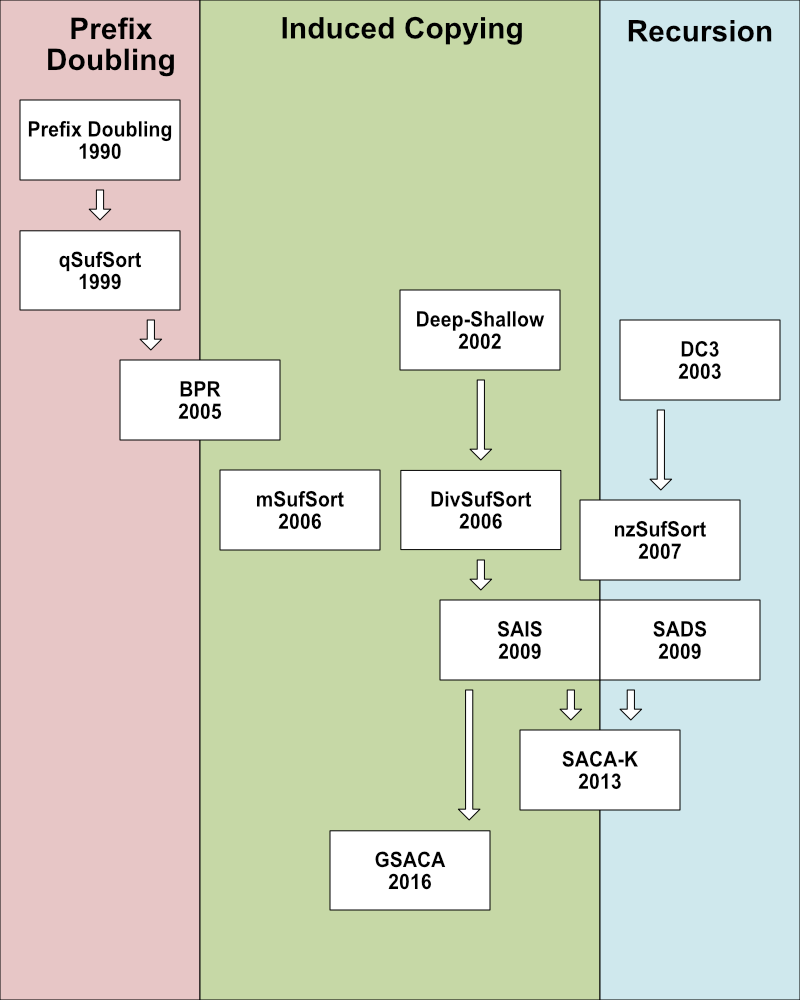
\includegraphics[width=\textwidth]{kapitel/5_saca_uebersicht/history/history3_eng.png}
    \caption{(partial) History of SACAs}
    \label{ea:fig:history}
\end{figure}

See Figure \ref{ea:fig:history} for a short summary of SACA history.
The different SACAs are divided into the three classes described above.
We now briefly explain the shown algorithms and their differences.

Prefix Doubling is a SACA which works purely by the above described method \emph{Doubling}.
In every iteration the \sa is refined and double the amount of characters are considered for sorting.
This directly influenced qSufSort, which improved its performance by using the \isa (inverse suffix arary) 
and subdividing suffixes into sorted and unsorted groups. 
BPR incorporated some ideas of inducing with prefix doubling and is therefore on the edge of those two paradigms.
Its inducing is based on the copy-technique by Seward~\cite{seward2000}.
This technique is also used by Deep-Shallow, which uses string-sorting instead of prefix doubling.
It influenced divsufsort, which sorts its RMS (rightmost S-Type) substrings before it completely sorts all RMS suffixes.
Given the correct order of the RMS suffixes, all remaining S-Type suffixes get induced in one and all L-Type suffixes in a second pass.
SAIS works by sorting all LMS (leftmost S-Type suffixes) in a recursion step before inducing the ordering of all suffixes in two passes similar to DivSufSort.
This is also done by SACA-K and GSACA, which are both similar to SAIS, but add some optimizations
(SACA-K for example doesn't use any extra space).
mSufSort is another inducing-SACA, but since it constructs the \isa instead of the \sa,
it's not derived from any other SACA.
The two other recursive SACAs are DC3 (which sorts $\frac{2}{3}$ of the suffixes in a recursion step), which utilizes the \emph{Difference Cover} concept to sort all suffixes beginning at positions $1$, $2$, $4$, $5$ and so on at first. After that, it uses this order to induce all suffixes beginning at positions $0$, $3$ and so on before these two are merged into the correct \sa.
nzSufSort sorts the S-Type suffixes by using the \emph{Difference Cover} concept before inducing the L-Type suffixes similar to SAIS in one pass. It was the first presented algorithm, which is \emph{optimal lightweight}. This means it has running time $\mathcal O (n)$ by using only constant extra space.

\section{Optimization Strategies}

As with most programs, much of the performance of SACAs is dependent on efficiently implementing these algorithms.
We therefore used some practical optimizations to the descriptions of the algorithms to improve performance.
The following is an incomplete list of tricks one can use to do so.

\subsection{Different bit lengths for the suffix array}

We implemented our SACAs with an exchangable suffix array index type, that is a different bit length for the indices in the suffix array.
With our current implementation it is possible to use 32, 40, 48 and 64 bit for the suffix array elements.
Since our tool supports a different output encoding (32 or 64 bit), we can save memory during construction regardless of the desired output length.
Keep in mind that since the 40- and 48-bit types are not standardized, their performance is inferior to those of 32- and 64- bit types.

\subsection{Cache-efficiency}

The most crucial part of optimizing a SACA is cache-efficiency, that is aiming for time-local and space-local memory access.
Since the \sa is a pseudo-random mutation of numbers, it can't be written cache-efficiently.
However, when implementing SACAs, avoiding unnecessary cache misses can significantly improve performance.

\subsection{Wordpacking}

To maximize throughput, multiple characters of the input (8 bit each) can be processed as a whole by
interpreting them as integer numbers (64 bit, or even up to 512 bit by using vector operations).
Algorithms using wordpacking techniques are the Osipov algorithm~\cite{osipovGPU},
Doubling~\cite{saca:11}, Discarding~\cite{saca:11} and qSufSort~\cite{saca:1}.

\subsection{Utilization of a GPU}

Since modern GPUs feature higher degrees of parallelism compared to CPUs due to their architecture,
we include a prefix doubling SACA which uses CUDA and the CUB-Framework to run on the GPU~\cite{osipovGPU}.
We show that this algorithm outperformes the parallel DivSufSort implementation,
although the required and available memory on current GPUs still restricts the algorithm to far smaller input sizes than CPU SACAs are capable of.
Further research of GPU SACAs should be considered,
as we could hardly find any (working) reference algorithms to compare our implementation with, 
% Das hier sollte als Allgemeinwissen klar sein:
and development of GPUs shows higher performance improvements than CPU development in certain workloads.

\subsection{Sorting Algorithms}

\begin{table}[!t]
    \centering
    \begin{tabular}{ll}
        \toprule
        Operating System     & GNU/Linux \\
        Kernel Version       & \#1 SMP Wed Sep 26 15:12:11 UTC 2018 \\
        \midrule
        Architecture:        & x86\_64 \\
        CPU op-mode(s):      & 32-bit, 64-bit \\
        CPU(s):              & 20 \\
        Thread(s) per core:  & 1 \\
        Core(s) per socket:  & 10 \\
        Socket(s):           & 2 \\
        Model name:          & Intel(R) Xeon(R) CPU E5-2640 v4 @ 2.40GHz \\
        CPU max MHz:         & 3400.0000 \\
        CPU min MHz:         & 1200.0000 \\
        L1d cache:           & 32K \\
        L1i cache:           & 32K \\
        L2 cache:            & 256K \\
        L3 cache:            & 25600K \\
        \midrule
        Memory Size          & 64GiB \\
        \bottomrule
    \end{tabular}
    \caption{Configuration of compute nodes used to run the SACAs in this evaluation. These nodes are part of the LiDO3 compute cluster~\cite{lido3} at TU Dortmund.}
    \label{ea:lido}
\end{table}

Many SACAs use sorting algorithms at some point. For the benchmark a variety of sorting algorithms were implemented so that all SACAs can use them.
We include some versions of quicksort, bucketsort and radixsort.
This is especially interesting for naive parallelization, where one may just switch from a sequential sorting algorithm to a parallel one
and thereby improve performance.
Besides our own implemented sorting algorithms some external sorting algorithms are also included.
Most of those external sorting algorithms are made for parallel use.

\subsubsection{Binary vs. ternary comparison-based sort}

Multiple versions of quicksort are implemented:
Two of them are introsort~\cite{Musser97} and ternary quicksort~\cite{ternary_quicksort}.
It has been shown that the binary sorting procedure is faster,
if there are no equal elements in the set to be sorted~\cite{saca:4,ternary_quicksort};
otherwise, the ternary version is faster~\cite{ternary_quicksort}.
We therefore chose the best option for the required use-case.

\section{Evaluation}

Evaluation of both the sequential SACAs, including the reference algorithms, as well as of the parallel SACAs is done on LiDO3~\cite{lido3}.
We evaluate the performance of the chosen SACAs on an identical test system, the specifications of which are described in \cref{ea:lido}.
This enables us to directly compare these algorithms in terms of runtime performance and memory consumption.
We set an arbitrary limit of 2 hours of runtime as well as 60 GiB of used system memory.
Our experiment texts are \texttt{wiki.txt}, \texttt{dna.txt} and \texttt{commoncrawl.txt}:
%
\begin{description}
    \item[\texttt{wiki.txt}] An XML-dump of the recent wikipedia database.
    \item[\texttt{dna.txt}] A version of the 1000 Genome Project~\cite{1000genomeproject}, which has been stripped from any characters but ACGT.
    \item[\texttt{commoncrawl.txt}] A subset of the Commoncrawl dataset~\cite{commoncrawl}, which has been cleaned up to contain only ASCII characters.
\end{description}

\subsection{Evaluation (sequential)}

In the Figures \ref{ea:runtime-all-ref-0} to \ref{ea:runtime-all-ref-2} we show the performance of
the implementations of different SACAs on a 1600 MiB prefix of the three texts.

The clear winners in all three cases is divsufsort, followed by BPR, SAIS-Lite
\footnote{divsufsort and SAIS-Lite both are optimized implementations by Yuta Mori~\cite{saca:5}.} and Deep-Shallow.
In terms of memory consumption, divsufsort and SACA-K are the two best algorithms since they use no extra space,
follwed by Deep-Shallow, which uses very little extra space.
The worst algorithm in both runtime performance as well as memory consumption is in all three cases the reference implementation of DC3,
which is followed by SADS (a variant of SAIS~\cite{saca:6}) in terms of performance and BPR in terms of memory consumption.
However, caused by source code incompatibilities,
memory utilization for BPR is not intuitively comparable to other algorithms as we are only able measure absolute memory
but not extra memory for this specific algorithm\footnote{It uses an auxiliary array the same size as the suffix array.}.
The runtime performance and memory consumption of the DC3 implementation is not well optimized by its authors~\cite{saca:9}.

The algorithms MSufSort, SACA-K, qsufsort, SAIS and GSACA share the mid field in terms of runtime performance.
Notable is the low memory consumption of SAIS and SACA-K, which only use some and none extra memory respectively.

\todo{800mb plots einbinden}

% IMPORT-DATA stats_parallel 7_messergebnisse/ergebnisse_parallel/result_weakscale.txt
% IMPORT-DATA results_sequential 7_messergebnisse/ergebnisse_sequentiell/results.txt

\begin{figure}[!ht]
    \textbf{Configuration} \hfill Input file: wiki.txt \hfill Prefix size: 1600\,MiB \\ Model name: Intel\textsuperscript{\textregistered} Xeon\textsuperscript{\textregistered} CPU E5-2640 v4 @ 2.40GHz
    \centering\small
    \begin{tikzpicture}[trim axis left]
        \begin{axis}[batchTimePlot,
            cycle list name={exotic},
            legend to name=ea-runtime-all-ref-0,
            width=\textwidth,
            height=60mm,
            xtick style = {draw=none},
            xticklabel pos=upper,
            title={},
            bar width=12pt,
            ylabel={\sa construction time [min]},
            legend style={
                /tikz/every even column/.append style={column sep=0.5cm,black},
                /tikz/every even column/.append style={black},
            },
            legend columns=2,
            symbolic x coords={ wiki.txt },
            every node near coord/.append style={color=black, rotate=90, anchor=west},
            ]

            %% MULTIPLOT(algo) SELECT algo, REPLACE(input, "_", "\_") AS x, time/1000/60 AS y
            %% FROM ( 
            %% SELECT algo, input, sacheck, MEDIAN(memFinal) AS memFinal, MEDIAN(memOff) AS memOff, AVG(memPeak) AS memPeak, prefix, rep_id, MEDIAN(time) AS time FROM results_sequential GROUP BY algo, input, prefix, rep_id
            %% ) WHERE input="wiki.txt" AND prefix=838860800 AND sacheck="ok"
            %% AND (algo LIKE "%_ref%" AND NOT algo LIKE "%par")
            %% AND rep_id=1 GROUP BY MULTIPLOT,x ORDER BY y
            \addplot coordinates { (wiki.txt,1.73052) };
            \addlegendentry{algo=DivSufSort\_ref};
            \addplot coordinates { (wiki.txt,2.75402) };
            \addlegendentry{algo=BPR\_ref};
            \addplot coordinates { (wiki.txt,2.77311) };
            \addlegendentry{algo=Deep-Shallow\_ref};
            \addplot coordinates { (wiki.txt,2.8182) };
            \addlegendentry{algo=SAIS-LITE\_ref};
            \addplot coordinates { (wiki.txt,4.35543) };
            \addlegendentry{algo=MSufSort\_ref};
            \addplot coordinates { (wiki.txt,5.17338) };
            \addlegendentry{algo=SACA-K\_ref};
            \addplot coordinates { (wiki.txt,6.1854) };
            \addlegendentry{algo=qsufsort\_ref};
            \addplot coordinates { (wiki.txt,7.28537) };
            \addlegendentry{algo=SAIS\_ref};
            \addplot coordinates { (wiki.txt,7.31669) };
            \addlegendentry{algo=GSACA\_ref};
            \addplot coordinates { (wiki.txt,9.19736) };
            \addlegendentry{algo=SADS\_ref};
            \addplot coordinates { (wiki.txt,23.235) };
            \addlegendentry{algo=DC3\_ref};

        \end{axis}
    \end{tikzpicture}
    \begin{tikzpicture}[trim axis left]
        \begin{axis}[batchTimePlot,
            cycle list name={exotic},
            width=\textwidth,
            height=60mm,
            xtick style = {draw=none},
            y dir=reverse,
            title={},
            bar width=12pt,
            ylabel={Extra Memory [GiB]},
            legend style={
                /tikz/every even column/.append style={column sep=0.5cm,black},
                /tikz/every even column/.append style={black},
            },
            legend columns=2,
            symbolic x coords={ wiki.txt },
            every node near coord/.append style={color=black, rotate=90, anchor=east, /pgf/number format/fixed},
            ]

            %% MULTIPLOT(algo) SELECT algo, REPLACE(input, "_", "\_") AS x, memPeak/1024/1024/1024 AS y
            %% FROM ( 
            %% SELECT algo, input, sacheck, MEDIAN(memFinal) AS memFinal, MEDIAN(memOff) AS memOff, AVG(memPeak) AS memPeak, prefix, rep_id, MEDIAN(time) AS time FROM results_sequential GROUP BY algo, input, prefix, rep_id
            %% ) WHERE input="wiki.txt" AND prefix=838860800 AND sacheck="ok"
            %% AND (algo LIKE "%_ref%" AND NOT algo LIKE "%par")
            %% AND rep_id=1 GROUP BY MULTIPLOT,x ORDER BY time
            \addplot coordinates { (wiki.txt,0.000249021) };
            \addlegendentry{algo=DivSufSort\_ref};
            \addplot coordinates { (wiki.txt,13.3493) };
            \addlegendentry{algo=BPR\_ref};
            \addplot coordinates { (wiki.txt,0.00939793) };
            \addlegendentry{algo=Deep-Shallow\_ref};
            \addplot coordinates { (wiki.txt,3.125) };
            \addlegendentry{algo=SAIS-LITE\_ref};
            \addplot coordinates { (wiki.txt,3.22572) };
            \addlegendentry{algo=MSufSort\_ref};
            \addplot coordinates { (wiki.txt,7.82311e-07) };
            \addlegendentry{algo=SACA-K\_ref};
            \addplot coordinates { (wiki.txt,12.5) };
            \addlegendentry{algo=qsufsort\_ref};
            \addplot coordinates { (wiki.txt,0.269095) };
            \addlegendentry{algo=SAIS\_ref};
            \addplot coordinates { (wiki.txt,9.375) };
            \addlegendentry{algo=GSACA\_ref};
            \addplot coordinates { (wiki.txt,0.360081) };
            \addlegendentry{algo=SADS\_ref};
            \addplot coordinates { (wiki.txt,18.3842) };
            \addlegendentry{algo=DC3\_ref};

            \legend{}
        \end{axis}
    \end{tikzpicture}

    \medskip
    \ref{ea-runtime-all-ref-0}

    \caption{Comparison of the in \sacabench included reference implementations of SACAs, including time and memory consumption: wiki.txt}
    \label{ea:runtime-all-ref-0}
\end{figure}

\begin{figure}[!ht]
    \textbf{Configuration} \hfill Input file: dna.txt \hfill Prefix size: 1600\,MiB \\ Model name: Intel\textsuperscript{\textregistered} Xeon\textsuperscript{\textregistered} CPU E5-2640 v4 @ 2.40GHz
    \centering\small
    \begin{tikzpicture}[trim axis left]
        \begin{axis}[batchTimePlot,
            cycle list name={exotic},
            legend to name=ea-runtime-all-ref-1,
            width=\textwidth,
            height=60mm,
            xtick style = {draw=none},
            xticklabel pos=upper,
            title={},
            bar width=12pt,
            ylabel={\sa construction time [min]},
            legend style={
                /tikz/every even column/.append style={column sep=0.5cm,black},
                /tikz/every even column/.append style={black},
            },
            legend columns=2,
            symbolic x coords={ dna.txt },
            every node near coord/.append style={color=black, rotate=90, anchor=west},
            ]

            %% MULTIPLOT(algo) SELECT algo, REPLACE(input, "_", "\_") AS x, time/1000/60 AS y
            %% FROM ( 
            %% SELECT algo, input, sacheck, MEDIAN(memFinal) AS memFinal, MEDIAN(memOff) AS memOff, AVG(memPeak) AS memPeak, prefix, rep_id, MEDIAN(time) AS time FROM results_sequential GROUP BY algo, input, prefix, rep_id
            %% ) WHERE input="dna.txt" AND prefix=838860800 AND sacheck="ok"
            %% AND (algo LIKE "%_ref%" AND NOT algo LIKE "%par")
            %% AND rep_id=1 GROUP BY MULTIPLOT,x ORDER BY y
            \addplot coordinates { (dna.txt,2.05917) };
            \addlegendentry{algo=DivSufSort\_ref};
            \addplot coordinates { (dna.txt,2.71512) };
            \addlegendentry{algo=SAIS-LITE\_ref};
            \addplot coordinates { (dna.txt,2.89482) };
            \addlegendentry{algo=Deep-Shallow\_ref};
            \addplot coordinates { (dna.txt,2.99629) };
            \addlegendentry{algo=BPR\_ref};
            \addplot coordinates { (dna.txt,4.34736) };
            \addlegendentry{algo=MSufSort\_ref};
            \addplot coordinates { (dna.txt,4.91973) };
            \addlegendentry{algo=SACA-K\_ref};
            \addplot coordinates { (dna.txt,5.44533) };
            \addlegendentry{algo=qsufsort\_ref};
            \addplot coordinates { (dna.txt,6.28076) };
            \addlegendentry{algo=GSACA\_ref};
            \addplot coordinates { (dna.txt,6.79781) };
            \addlegendentry{algo=SAIS\_ref};
            \addplot coordinates { (dna.txt,8.94179) };
            \addlegendentry{algo=SADS\_ref};
            \addplot coordinates { (dna.txt,16.6623) };
            \addlegendentry{algo=DC3\_ref};

        \end{axis}
    \end{tikzpicture}
    \begin{tikzpicture}[trim axis left]
        \begin{axis}[batchTimePlot,
            cycle list name={exotic},
            width=\textwidth,
            height=60mm,
            xtick style = {draw=none},
            y dir=reverse,
            title={},
            bar width=12pt,
            ylabel={Extra Memory [GiB]},
            legend style={
                /tikz/every even column/.append style={column sep=0.5cm,black},
                /tikz/every even column/.append style={black},
            },
            legend columns=2,
            symbolic x coords={ dna.txt },
            every node near coord/.append style={color=black, rotate=90, anchor=east, /pgf/number format/fixed},
            ]

            %% MULTIPLOT(algo) SELECT algo, REPLACE(input, "_", "\_") AS x, memPeak/1024/1024/1024 AS y
            %% FROM ( 
            %% SELECT algo, input, sacheck, MEDIAN(memFinal) AS memFinal, MEDIAN(memOff) AS memOff, AVG(memPeak) AS memPeak, prefix, rep_id, MEDIAN(time) AS time FROM results_sequential GROUP BY algo, input, prefix, rep_id
            %% ) WHERE input="dna.txt" AND prefix=838860800 AND sacheck="ok"
            %% AND (algo LIKE "%_ref%" AND NOT algo LIKE "%par")
            %% AND rep_id=1 GROUP BY MULTIPLOT,x ORDER BY time
            \addplot coordinates { (dna.txt,0.000249021) };
            \addlegendentry{algo=DivSufSort\_ref};
            \addplot coordinates { (dna.txt,3.125) };
            \addlegendentry{algo=SAIS-LITE\_ref};
            \addplot coordinates { (dna.txt,0.00937501) };
            \addlegendentry{algo=Deep-Shallow\_ref};
            \addplot coordinates { (dna.txt,13.2814) };
            \addlegendentry{algo=BPR\_ref};
            \addplot coordinates { (dna.txt,3.92618) };
            \addlegendentry{algo=MSufSort\_ref};
            \addplot coordinates { (dna.txt,1.86265e-08) };
            \addlegendentry{algo=SACA-K\_ref};
            \addplot coordinates { (dna.txt,12.5) };
            \addlegendentry{algo=qsufsort\_ref};
            \addplot coordinates { (dna.txt,9.375) };
            \addlegendentry{algo=GSACA\_ref};
            \addplot coordinates { (dna.txt,0.235499) };
            \addlegendentry{algo=SAIS\_ref};
            \addplot coordinates { (dna.txt,0.334526) };
            \addlegendentry{algo=SADS\_ref};
            \addplot coordinates { (dna.txt,17.5154) };
            \addlegendentry{algo=DC3\_ref};

            \legend{}
        \end{axis}
    \end{tikzpicture}
    \medskip
    \ref{ea-runtime-all-ref-1}
    \caption{Comparison of the in \sacabench included reference implementations of SACAs, including time and memory consumption: dna.txt}
    \label{ea:runtime-all-ref-1}
\end{figure}

\begin{figure}[!ht]
    \textbf{Configuration} \hfill Input file: commoncrawl.txt \hfill Prefix size: 1600\,MiB \\ Model name: Intel\textsuperscript{\textregistered} Xeon\textsuperscript{\textregistered} CPU E5-2640 v4 @ 2.40GHz
    \centering\small
    \begin{tikzpicture}[trim axis left]
        \begin{axis}[batchTimePlot,
            cycle list name={exotic},
            legend to name=ea-runtime-all-ref-2,
            width=\textwidth,
            height=60mm,
            xtick style = {draw=none},
            xticklabel pos=upper,
            title={},
            bar width=12pt,
            ylabel={\sa construction time [min]},
            legend style={
                /tikz/every even column/.append style={column sep=0.5cm,black},
                /tikz/every even column/.append style={black},
            },
            legend columns=2,
            symbolic x coords={ commoncrawl.txt },
            every node near coord/.append style={color=black, rotate=90, anchor=west},
            ]

            %% MULTIPLOT(algo) SELECT algo, REPLACE(input, "_", "\_") AS x, time/1000/60 AS y
            %% FROM ( 
            %% SELECT algo, input, sacheck, MEDIAN(memFinal) AS memFinal, MEDIAN(memOff) AS memOff, AVG(memPeak) AS memPeak, prefix, rep_id, MEDIAN(time) AS time FROM results_sequential GROUP BY algo, input, prefix, rep_id
            %% ) WHERE input="commoncrawl.txt" AND prefix=838860800 AND sacheck="ok"
            %% AND (algo LIKE "%_ref%" AND NOT algo LIKE "%par")
            %% AND rep_id=1 GROUP BY MULTIPLOT,x ORDER BY y
            \addplot coordinates { (commoncrawl.txt,1.5745) };
            \addlegendentry{algo=DivSufSort\_ref};
            \addplot coordinates { (commoncrawl.txt,2.28537) };
            \addlegendentry{algo=SAIS-LITE\_ref};
            \addplot coordinates { (commoncrawl.txt,2.889) };
            \addlegendentry{algo=BPR\_ref};
            \addplot coordinates { (commoncrawl.txt,3.24651) };
            \addlegendentry{algo=Deep-Shallow\_ref};
            \addplot coordinates { (commoncrawl.txt,3.33703) };
            \addlegendentry{algo=MSufSort\_ref};
            \addplot coordinates { (commoncrawl.txt,4.43887) };
            \addlegendentry{algo=SACA-K\_ref};
            \addplot coordinates { (commoncrawl.txt,5.9169) };
            \addlegendentry{algo=SAIS\_ref};
            \addplot coordinates { (commoncrawl.txt,6.09891) };
            \addlegendentry{algo=GSACA\_ref};
            \addplot coordinates { (commoncrawl.txt,6.92753) };
            \addlegendentry{algo=qsufsort\_ref};
            \addplot coordinates { (commoncrawl.txt,7.57719) };
            \addlegendentry{algo=SADS\_ref};
            \addplot coordinates { (commoncrawl.txt,22.2288) };
            \addlegendentry{algo=DC3\_ref};

        \end{axis}
    \end{tikzpicture}
    \begin{tikzpicture}[trim axis left]
        \begin{axis}[batchTimePlot,
            cycle list name={exotic},
            width=\textwidth,
            height=60mm,
            xtick style = {draw=none},
            y dir=reverse,
            title={},
            bar width=12pt,
            ylabel={Extra Memory [GiB]},
            legend style={
                /tikz/every even column/.append style={column sep=0.5cm,black},
                /tikz/every even column/.append style={black},
            },
            legend columns=2,
            symbolic x coords={ commoncrawl.txt },
            every node near coord/.append style={color=black, rotate=90, anchor=east, /pgf/number format/fixed},
            ]

            %% MULTIPLOT(algo) SELECT algo, REPLACE(input, "_", "\_") AS x, memPeak/1024/1024/1024 AS y
            %% FROM ( 
            %% SELECT algo, input, sacheck, MEDIAN(memFinal) AS memFinal, MEDIAN(memOff) AS memOff, AVG(memPeak) AS memPeak, prefix, rep_id, MEDIAN(time) AS time FROM results_sequential GROUP BY algo, input, prefix, rep_id
            %% ) WHERE input="commoncrawl.txt" AND prefix=838860800 AND sacheck="ok"
            %% AND (algo LIKE "%_ref%" AND NOT algo LIKE "%par")
            %% AND rep_id=1 GROUP BY MULTIPLOT,x ORDER BY time
            \addplot coordinates { (commoncrawl.txt,0.000249021) };
            \addlegendentry{algo=DivSufSort\_ref};
            \addplot coordinates { (commoncrawl.txt,3.125) };
            \addlegendentry{algo=SAIS-LITE\_ref};
            \addplot coordinates { (commoncrawl.txt,13.3868) };
            \addlegendentry{algo=BPR\_ref};
            \addplot coordinates { (commoncrawl.txt,0.00945246) };
            \addlegendentry{algo=Deep-Shallow\_ref};
            \addplot coordinates { (commoncrawl.txt,3.15495) };
            \addlegendentry{algo=MSufSort\_ref};
            \addplot coordinates { (commoncrawl.txt,9.05246e-07) };
            \addlegendentry{algo=SACA-K\_ref};
            \addplot coordinates { (commoncrawl.txt,0.26491) };
            \addlegendentry{algo=SAIS\_ref};
            \addplot coordinates { (commoncrawl.txt,9.375) };
            \addlegendentry{algo=GSACA\_ref};
            \addplot coordinates { (commoncrawl.txt,12.5) };
            \addlegendentry{algo=qsufsort\_ref};
            \addplot coordinates { (commoncrawl.txt,0.338007) };
            \addlegendentry{algo=SADS\_ref};
            \addplot coordinates { (commoncrawl.txt,18.6777) };
            \addlegendentry{algo=DC3\_ref};

            \legend{}
        \end{axis}
    \end{tikzpicture}
    \medskip
    \ref{ea-runtime-all-ref-2}
    \caption{Comparison of the in \sacabench included reference implementations of SACAs, including time and memory consumption: commoncrawl.txt}
    \label{ea:runtime-all-ref-2}
\end{figure}

\FloatBarrier

\subsection{Evaluation (parallel)}

In this section we will compare the performance of the runtime and memory performance of the included parallel SACAs.
These are variants of the sequential algorithms, that were mostly naively parallelized, with the exception of parallel SAIS
\footnote{This algorithm uses read/write buffers and a parallel pipeline based on work of Lao et al~\cite{psais}.}.

\begin{figure}[!ht]
    \centering
    \begin{tikzpicture}[trim axis left]
        \begin{axis}[
                name=axis1,
                cycle list name={exoticlines},
                width=\textwidth,
                height=60mm,
                title={wiki.txt},
                xlabel={num threads, input size [200\,MB]},
                ylabel={SA construction time [min]},
                legend columns=2,
                legend to name=ea-legend-par-all-0,
                legend style={
                    /tikz/every even column/.append style={column sep=0.5cm,black},
                    /tikz/every even column/.append style={black},
                },
            ]

            %% MULTIPLOT(algo) SELECT thread_count AS x, time/1000/60 AS y, MULTIPLOT
            %% FROM (
            %% SELECT algo, input, MEDIAN(memFinal) AS memFinal, MEDIAN(memOff) AS memOff, AVG(memPeak) AS memPeak, prefix, rep, thread_count, MEDIAN(time) AS time, sacheck FROM stats_parallel GROUP BY algo, input, prefix, rep, thread_count
            %% ) WHERE input="wiki.txt" AND sacheck="ok"
            %% AND (algo="BPR_par" OR algo="DC3-Parallel-V2" OR algo="NaivParallel" OR algo="Deep-Shallow_par" OR algo="Discarding2Parallel" OR algo="Discarding4Parallel" OR algo="PARALLEL_SAIS")
            %% GROUP BY MULTIPLOT,x ORDER BY MULTIPLOT,x
            \addplot coordinates { (1,0.543257) (2,1.04248) (4,2.69455) (8,5.00914) (12,8.55647) (16,12.5204) };
            \addlegendentry{algo=BPR\_par};
            \addplot coordinates { (1,3.09365) (2,4.11916) (4,5.55123) (8,7.75629) };
            \addlegendentry{algo=DC3-Parallel-V2};
            \addplot coordinates { (1,1.41234) (2,1.79674) (4,2.28839) (8,3.29598) (12,4.53346) (16,5.42954) (20,6.48599) };
            \addlegendentry{algo=Deep-Shallow\_par};
            \addplot coordinates { (1,3.20359) (2,3.69207) (4,4.44643) (8,5.90081) };
            \addlegendentry{algo=Discarding2Parallel};
            \addplot coordinates { (1,2.32532) (2,2.82934) (4,3.37798) (8,4.41391) };
            \addlegendentry{algo=Discarding4Parallel};
            \addplot coordinates { (1,2.71662) (2,3.54087) (4,4.03271) (8,4.7199) (12,5.55871) (16,5.86449) };
            \addlegendentry{algo=NaivParallel};
            \addplot coordinates { (1,1.07199) (2,2.15225) (4,4.661) (8,10.5053) };
            \addlegendentry{algo=PARALLEL\_SAIS};
        \end{axis}
    \end{tikzpicture}
    \par\bigskip
    \begin{tikzpicture}[trim axis left]
        \begin{axis}[
                cycle list name={exoticlines},
                at={(axis1.outer north east)},
                anchor=outer north west,
                name=axis2,
                width=\textwidth,
                height=60mm,
                title={wiki.txt},
                xlabel={num threads, input size [200\,MB]},
                ylabel={Extra Memory [GiB]},
            ]

            %% MULTIPLOT(algo) SELECT thread_count AS x, memPeak/1024/1024/1024 AS y, MULTIPLOT
            %% FROM (
            %% SELECT algo, input, MEDIAN(memFinal) AS memFinal, MEDIAN(memOff) AS memOff, AVG(memPeak) AS memPeak, prefix, rep, thread_count, MEDIAN(time) AS time, sacheck FROM stats_parallel GROUP BY algo, input, prefix, rep, thread_count
            %% ) WHERE input="wiki.txt" AND sacheck="ok"
            %% AND (algo="BPR_par" OR algo="DC3-Parallel-V2" OR algo="NaivParallel" OR algo="Deep-Shallow_par" OR algo="Discarding2Parallel" OR algo="Discarding4Parallel" OR algo="PARALLEL_SAIS")
            %% GROUP BY MULTIPLOT,x ORDER BY MULTIPLOT,x
            \addplot coordinates { (1,0.951951) (2,1.7332) (4,3.4355) (8,6.83651) (12,19.647) (16,26.173) };
            \addlegendentry{algo=BPR\_par};
            \addplot coordinates { (1,3.10468) (2,8.33334) (4,16.6667) (8,31.9445) };
            \addlegendentry{algo=DC3-Parallel-V2};
            \addplot coordinates { (1,0.00319003) (2,0.00532148) (4,0.00959451) (8,0.0183557) (12,0.0497788) (16,0.0630637) (20,0.0779177) };
            \addlegendentry{algo=Deep-Shallow\_par};
            \addplot coordinates { (1,2.34575) (2,4.69158) (4,9.38307) (8,18.766) };
            \addlegendentry{algo=Discarding2Parallel};
            \addplot coordinates { (1,3.90825) (2,7.81659) (4,15.6331) (8,31.2661) };
            \addlegendentry{algo=Discarding4Parallel};
            \addplot coordinates { (1,0.0) (2,1.5625) (4,3.12501) (8,6.25002) (12,18.75) (16,25) };
            \addlegendentry{algo=NaivParallel};
            \addplot coordinates { (1,0.416671) (2,0.524891) (4,0.731684) (8,1.10245) };
            \addlegendentry{algo=PARALLEL\_SAIS};

            \legend{}
        \end{axis}
    \end{tikzpicture}

    \medskip
    \ref{ea-legend-par-all-0}
    \caption{Vergleich der parallelen Implementierungen mit Laufzeit und Speicherbedarf auf wiki.txt}
    \label{ea:fig-par-all-0}
\end{figure}

\begin{figure}[!ht]
    \centering
    \begin{tikzpicture}[trim axis left]
        \begin{axis}[
                name=axis1,
                cycle list name={exoticlines},
                width=\textwidth,
                height=60mm,
                title={dna.txt},
                xlabel={num threads, input size [200\,MB]},
                ylabel={SA construction time [min]},
                legend columns=2,
                legend to name=ea-legend-par-all-1,
                legend style={
                    /tikz/every even column/.append style={column sep=0.5cm,black},
                    /tikz/every even column/.append style={black},
                },
            ]

            %% MULTIPLOT(algo) SELECT thread_count AS x, time/1000/60 AS y, MULTIPLOT
            %% FROM (
            %% SELECT algo, input, MEDIAN(memFinal) AS memFinal, MEDIAN(memOff) AS memOff, AVG(memPeak) AS memPeak, prefix, rep, thread_count, MEDIAN(time) AS time, sacheck FROM stats_parallel GROUP BY algo, input, prefix, rep, thread_count
            %% ) WHERE input="dna.txt" AND sacheck="ok"
            %% AND (algo="BPR_par" OR algo="DC3-Parallel-V2" OR algo="NaivParallel" OR algo="Deep-Shallow_par" OR algo="Discarding2Parallel" OR algo="Discarding4Parallel" OR algo="PARALLEL_SAIS")
            %% GROUP BY MULTIPLOT,x ORDER BY MULTIPLOT,x
            \addplot coordinates { (1,0.569637) (2,1.09372) (4,2.16083) (8,4.4065) (12,8.71249) (16,11.9082) };
            \addlegendentry{algo=BPR\_par};
            \addplot coordinates { (1,3.02187) (2,3.97795) (4,5.28252) (8,7.08082) };
            \addlegendentry{algo=DC3-Parallel-V2};
            \addplot coordinates { (1,1.84653) (2,2.47075) (4,3.2711) (8,4.23853) (12,5.92934) (16,9.05611) (20,10.8896) };
            \addlegendentry{algo=Deep-Shallow\_par};
            \addplot coordinates { (1,3.2561) (2,3.83204) (4,4.51572) (8,5.42115) };
            \addlegendentry{algo=Discarding2Parallel};
            \addplot coordinates { (1,2.50936) (2,3.04948) (4,3.62786) (8,4.52356) };
            \addlegendentry{algo=Discarding4Parallel};
            \addplot coordinates { (1,3.06848) (2,4.3148) (4,4.73058) (8,5.05918) (12,5.68415) (16,5.68597) };
            \addlegendentry{algo=NaivParallel};
            \addplot coordinates { (1,1.11013) (2,2.02917) (4,4.40177) (8,9.565) };
            \addlegendentry{algo=PARALLEL\_SAIS};

        \end{axis}
    \end{tikzpicture}
    \par\bigskip
    \begin{tikzpicture}[trim axis left]
        \begin{axis}[
                cycle list name={exoticlines},
                at={(axis1.outer north east)},
                anchor=outer north west,
                name=axis2,
                width=\textwidth,
                height=60mm,
                title={dna.txt},
                xlabel={num threads, input size [200\,MB]},
                ylabel={Extra Memory [GiB]},
            ]

            %% MULTIPLOT(algo) SELECT thread_count AS x, memPeak/1024/1024/1024 AS y, MULTIPLOT
            %% FROM (
            %% SELECT algo, input, MEDIAN(memFinal) AS memFinal, MEDIAN(memOff) AS memOff, AVG(memPeak) AS memPeak, prefix, rep, thread_count, MEDIAN(time) AS time, sacheck FROM stats_parallel GROUP BY algo, input, prefix, rep, thread_count
            %% ) WHERE input="dna.txt" AND sacheck="ok"
            %% AND (algo="BPR_par" OR algo="DC3-Parallel-V2" OR algo="NaivParallel" OR algo="Deep-Shallow_par" OR algo="Discarding2Parallel" OR algo="Discarding4Parallel" OR algo="PARALLEL_SAIS")
            %% GROUP BY MULTIPLOT,x ORDER BY MULTIPLOT,x
            \addplot coordinates { (1,0.783537) (2,1.56479) (4,3.12762) (8,6.25495) (12,18.7576) (16,25.0099) };
            \addlegendentry{algo=BPR\_par};
            \addplot coordinates { (1,3.05641) (2,8.33334) (4,16.6667) (8,33.3333) };
            \addlegendentry{algo=DC3-Parallel-V2};
            \addplot coordinates { (1,0.00213599) (2,0.00426745) (4,0.00853033) (8,0.0170561) (12,0.0427683) (16,0.0569774) (20,0.0711839) };
            \addlegendentry{algo=Deep-Shallow\_par};
            \addplot coordinates { (1,2.34575) (2,4.69158) (4,9.38307) (8,18.766) };
            \addlegendentry{algo=Discarding2Parallel};
            \addplot coordinates { (1,3.90825) (2,7.81659) (4,15.6331) (8,31.2661) };
            \addlegendentry{algo=Discarding4Parallel};
            \addplot coordinates { (1,0.0) (2,1.5625) (4,3.12501) (8,6.25002) (12,18.75) (16,25) };
            \addlegendentry{algo=NaivParallel};
            \addplot coordinates { (1,0.399128) (2,0.48352) (4,0.654059) (8,1.0149) };
            \addlegendentry{algo=PARALLEL\_SAIS};

            \legend{}
        \end{axis}
    \end{tikzpicture}

    \medskip
    \ref{ea-legend-par-all-1}
    \caption{Vergleich der parallelen Implementierungen mit Laufzeit und Speicherbedarf auf dna.txt}
    \label{ea:fig-par-all-1}
\end{figure}

\begin{figure}[!ht]
    \centering
    \begin{tikzpicture}[trim axis left]
        \begin{axis}[
                name=axis1,
                cycle list name={exoticlines},
                width=\textwidth,
                height=60mm,
                title={commoncrawl.txt},
                xlabel={num threads, input size [200\,MB]},
                ylabel={SA construction time [min]},
                legend columns=2,
                legend to name=ea-legend-par-all-2,
                legend style={
                    /tikz/every even column/.append style={column sep=0.5cm,black},
                    /tikz/every even column/.append style={black},
                },
            ]

            %% MULTIPLOT(algo) SELECT thread_count AS x, time/1000/60 AS y, MULTIPLOT
            %% FROM (
            %% SELECT algo, input, MEDIAN(memFinal) AS memFinal, MEDIAN(memOff) AS memOff, AVG(memPeak) AS memPeak, prefix, rep, thread_count, MEDIAN(time) AS time, sacheck FROM stats_parallel GROUP BY algo, input, prefix, rep, thread_count
            %% ) WHERE input="commoncrawl.txt" AND sacheck="ok"
            %% AND (algo="BPR_par" OR algo="DC3-Parallel-V2" OR algo="NaivParallel" OR algo="Deep-Shallow_par" OR algo="Discarding2Parallel" OR algo="Discarding4Parallel" OR algo="PARALLEL_SAIS")
            %% GROUP BY MULTIPLOT,x ORDER BY MULTIPLOT,x
            \addplot coordinates { (1,0.469155) (2,0.910706) (4,1.81015) (8,3.76797) (12,7.48885) (16,11.141) };
            \addlegendentry{algo=BPR\_par};
            \addplot coordinates { (1,2.95908) (2,3.97025) (4,5.25151) (8,7.6797) };
            \addlegendentry{algo=DC3-Parallel-V2};
            \addplot coordinates { (1,7.83762) (2,7.19017) (4,9.73639) };
            \addlegendentry{algo=Deep-Shallow\_par};
            \addplot coordinates { (1,5.61108) (2,6.40921) (4,7.93302) (8,10.0045) };
            \addlegendentry{algo=Discarding2Parallel};
            \addplot coordinates { (1,3.54234) (2,4.24778) (4,5.16101) (8,6.84444) };
            \addlegendentry{algo=Discarding4Parallel};
            \addplot coordinates { (1,7.15567) (2,7.39145) (4,8.81336) (8,11.3875) (12,13.2541) (16,15.516) };
            \addlegendentry{algo=NaivParallel};
            \addplot coordinates { (1,0.926488) (2,1.85933) (4,3.9815) (8,8.77113) };
            \addlegendentry{algo=PARALLEL\_SAIS};

        \end{axis}
    \end{tikzpicture}
    \par\bigskip
    \begin{tikzpicture}[trim axis left]
        \begin{axis}[
                cycle list name={exoticlines},
                at={(axis1.outer north east)},
                anchor=outer north west,
                name=axis2,
                width=\textwidth,
                height=60mm,
                title={commoncrawl.txt},
                xlabel={num threads, input size [200\,MB]},
                ylabel={Extra Memory [GiB]},
            ]

            %% MULTIPLOT(algo) SELECT thread_count AS x, memPeak/1024/1024/1024 AS y, MULTIPLOT
            %% FROM (
            %% SELECT algo, input, MEDIAN(memFinal) AS memFinal, MEDIAN(memOff) AS memOff, AVG(memPeak) AS memPeak, prefix, rep, thread_count, MEDIAN(time) AS time, sacheck FROM stats_parallel GROUP BY algo, input, prefix, rep, thread_count
            %% ) WHERE input="commoncrawl.txt" AND sacheck="ok"
            %% AND (algo="BPR_par" OR algo="DC3-Parallel-V2" OR algo="NaivParallel" OR algo="Deep-Shallow_par" OR algo="Discarding2Parallel" OR algo="Discarding4Parallel" OR algo="PARALLEL_SAIS")
            %% GROUP BY MULTIPLOT,x ORDER BY MULTIPLOT,x
            \addplot coordinates { (1,1.02691) (2,1.8241) (4,3.60609) (8,7.15872) (12,20.1398) (16,26.8174) };
            \addlegendentry{algo=BPR\_par};
            \addplot coordinates { (1,3.11898) (2,8.33334) (4,16.6667) (8,33.3334) };
            \addlegendentry{algo=DC3-Parallel-V2};
            \addplot coordinates { (1,0.00348096) (2,0.00567017) (4,0.0413734) };
            \addlegendentry{algo=Deep-Shallow\_par};
            \addplot coordinates { (1,2.34575) (2,4.69158) (4,9.38307) (8,18.766) };
            \addlegendentry{algo=Discarding2Parallel};
            \addplot coordinates { (1,3.90825) (2,7.81659) (4,15.6331) (8,31.2661) };
            \addlegendentry{algo=Discarding4Parallel};
            \addplot coordinates { (1,0.0) (2,1.5625) (4,3.12501) (8,6.25002) (12,18.75) (16,25) };
            \addlegendentry{algo=NaivParallel};
            \addplot coordinates { (1,0.410859) (2,0.513571) (4,0.698684) (8,1.0433) };
            \addlegendentry{algo=PARALLEL\_SAIS};

            \legend{}
        \end{axis}
    \end{tikzpicture}

    \medskip
    \ref{ea-legend-par-all-2}
    \caption{Vergleich der parallelen Implementierungen mit Laufzeit und Speicherbedarf auf commoncrawl.txt}
    \label{ea:fig-par-all-2}
\end{figure}

Contrary to the results of the sequential algorithms, the performance of the parallel SACAs differ widely between the input text.
For example, Deep-Shallow\_par is the best algorithm on \texttt{wiki.txt},
as it uses 0 extra memory and outperformes the other algorithms in terms of runtime.
However, it is surpassed on \texttt{dna.txt} by even the naive-parallel SACA and fails to compute the correct \sa on \texttt{commoncrawl.txt}.

Discarding4 has consistent runtime performance on all of the three texts but comes with a heavy memory pricetag.
Its memory comsumption is the same as for the parallel DC3 implementation,
which in turn has higher or equal runtime compared to Discarding4 on all three input texts.

Parallel BPR is the fastest algorithm on \texttt{commoncrawl.txt} and its memory consumption is similar to that of the naive parallel SACA.
It needs a lot more memory than parallel SACAs with almost no need for extra memory (Deep-Shallow\_par, pSAIS).

\todo{warum brechen da algos ab? (mb)}
\todo{warum brechen alle algos ab 8 kernen ab? (mb)}
\todo{sicherstellen dass mind eine ref drin ist (divsufsort par ref) (mb)}

\subsection{Evaluation (GPU)}

\begin{figure}[ht]
    \textbf{Configuration} \hfill Prefix size: 200\,MiB \\ Model name: Intel\textsuperscript{\textregistered} Xeon\textsuperscript{\textregistered} CPU E5-2640 v4 @ 2.40GHz\\
\textcolor{white}{h} \hspace{0.65cm}  NVIDIA\textsuperscript{\textregistered} Tesla K40 @ 2880 CUDA\textsuperscript{\textregistered} cores
    \centering\small
    \begin{tikzpicture}[trim axis left]
        \begin{axis}[batchTimePlot,
            cycle list name={exotic},
            legend to name=ea:runtime-gpu-0,
            width=\textwidth,
            height=50mm,
            xtick style = {draw=none},
            title={},
            bar width=12pt,
            ylabel={SA construction time [s]},
            legend style={
                /tikz/every even column/.append style={column sep=0.5cm,black},
                /tikz/every even column/.append style={black},
            },
            legend columns=2,
            symbolic x coords={ pc\_dblp.xml.200MB, pc\_dna.200MB, pc\_english.200MB, pc\_sources.200MB, pc\_proteins.200MB },
            every node near coord/.append style={color=black, rotate=90, anchor=west},
            ]

            %% MULTIPLOT(algo) SELECT algo, REPLACE(input, "_", "\_") AS x, time/1000 AS y
            %% FROM ( 
            %% SELECT algo, input, MEDIAN(memFinal) AS memFinal, MEDIAN(memOff) AS memOff, AVG(memPeak) AS memPeak, prefix, rep_id, MEDIAN(time) AS time FROM result_gpu GROUP BY algo, input, prefix, rep_id
            %% ) WHERE (input="pc_dblp.xml.200MB" OR input="pc_dna.200MB")
            %% AND rep_id=1 GROUP BY MULTIPLOT,x ORDER BY y
            \addplot coordinates { (pc\_dna.200MB,9.30329) (pc\_dblp.xml.200MB,11.5691) };
            \addlegendentry{algo=Osipov\_gpu};
            \addplot coordinates { (pc\_dblp.xml.200MB,18.7458) (pc\_dna.200MB,29.7007) };
            \addlegendentry{algo=DivSufSort\_par\_ref};
            \addplot coordinates { (pc\_dna.200MB,40.8382) (pc\_dblp.xml.200MB,54.6578) };
            \addlegendentry{algo=Osipov\_parallel};
        \end{axis}
    \end{tikzpicture}
    \medskip
    \ref{ea:runtime-gpu-0}
    \caption{Comparison of our parallel implementations of the Osipov algorithm for GPU and CPU and divsufsort by Mori on pc\_dna.200MB}
\label{ea:gpu_benchmark:1}
\end{figure}

\begin{figure}[ht]
    \textbf{Configuration} \hfill Prefix size: 200\,MiB \\ Model name: Intel\textsuperscript{\textregistered} Xeon\textsuperscript{\textregistered} CPU E5-2640 v4 @ 2.40GHz \\\textcolor{white}{h} \hspace{0.65cm}  NVIDIA\textsuperscript{\textregistered} Tesla K40 @ 2880 CUDA\textsuperscript{\textregistered} cores
    \centering\small
    \begin{tikzpicture}[trim axis left]
        \begin{axis}[batchTimePlot,
            cycle list name={exotic},
            legend to name=ea:runtime-gpu-1,
            width=\textwidth,
            height=50mm,
            xtick style = {draw=none},
            title={},
            bar width=12pt,
            ylabel={SA construction time [s]},
            legend style={
                /tikz/every even column/.append style={column sep=0.5cm,black},
                /tikz/every even column/.append style={black},
            },
            legend columns=2,
            symbolic x coords={ pc\_dblp.xml.200MB, pc\_dna.200MB, pc\_english.200MB, pc\_sources.200MB, pc\_proteins.200MB },
            every node near coord/.append style={color=black, rotate=90, anchor=west},
            ]

            %% MULTIPLOT(algo) SELECT algo, REPLACE(input, "_", "\_") AS x, time/1000 AS y
            %% FROM ( 
            %% SELECT algo, input, MEDIAN(memFinal) AS memFinal, MEDIAN(memOff) AS memOff, AVG(memPeak) AS memPeak, prefix, rep_id, MEDIAN(time) AS time FROM result_gpu GROUP BY algo, input, prefix, rep_id
            %% ) WHERE (input="pc_english.200MB" OR input="pc_proteins.200MB")
            %% GROUP BY MULTIPLOT,x ORDER BY y
            \addplot coordinates { (pc\_proteins.200MB,12.4394) (pc\_english.200MB,17.1103) };
            \addlegendentry{algo=Osipov\_gpu};
            \addplot coordinates { (pc\_proteins.200MB,23.5957) (pc\_english.200MB,25.0026) };
            \addlegendentry{algo=DivSufSort\_par\_ref};
            \addplot coordinates { (pc\_proteins.200MB,55.1025) (pc\_english.200MB,75.315) };
            \addlegendentry{algo=Osipov\_parallel};
        \end{axis}
    \end{tikzpicture}
    \medskip
    \ref{ea:runtime-gpu-1}
    \caption{Comparison of our parallel implementations of the Osipov algorithm for GPU and CPU and divsufsort by Mori on pc\_english.200MB}
\label{ea:gpu_benchmark:2}
\end{figure}
\FloatBarrier
Figures \ref{ea:gpu_benchmark:1} and \ref{ea:gpu_benchmark:2} show the runtime comparisons between the parallel version of Mori's DivSufSort and the variants of the Osipov prefix doubler implemented by us, both the parallel variant for the CPU and for the GPU. 

It can be seen here too that the DivSufSort on all four input texts is in part clearly superior to the other CPU implementation in terms of runtime. The situation is different in comparison to the GPU implementation: on all four input texts it achieves better runtimes than both CPU algorithms. On average this takes 12.6 seconds in our benchmarks, the DivSufSort 24.26 seconds and the CPU counterpart of the prefix doubler even 56.48 seconds. 
In addition, it can be observed that both the GPU-Osipov with 3.28 seconds and the parallel DivSufSort with 4.5 seconds have small standard deviations and therefore do not react disproportionately differently to different input texts. The CPU version of the Osipov algorithm, which has a standard deviation of 14.19 seconds for the four texts of the same size and thus comparatively large fluctuations in the runtime, has a different effect.

However, the high memory consumption of the Osipov algorithm is not evident from these graphs. The memory consumption of the Osipov implementations adds up to $28n$ ($20n$ for our implementation, approx. $8n$ for the radix location) and is thus significantly higher than that of the DivSufSort, which requires additional memory depending on the alphabet size $|\Sigma|$.

\section{Conclusion}

We introduced \sacabench, an extensive framework for benchmarking and comparing suffix array construction algorithms.
It includes a large set of publicly available SACAs as well as re-implementations%
\footnote{These re-implementations should be easier to understand than the reference implementations since they are heavily commented and written in modern C++.}
of these SACAs and simplifies the evaluation of new SACAs.
The code is written in modern C++ and well documented and can therefore be helpful in understanding the included algorithms.
We also include several parallel SACAs as well as parallel reference implementations.
In our evaluation we compared the performance of the SACAs on different texts of different type and size.
We can confirm divsufsort's dominance on most of the tested texts.

Our parallel implementations scale well up to 20 CPU cores and the GPU-SACA (Osipov/Prefix Doubling) is faster than the parallel divsufsort.
We show that shared-memory parallelization is a fruitful approach to suffix sorting
and can be used to accelerate construction of medium to large size suffix arrays.
Since there are some texts on which the \sa can't be calculated by any of our included algorithms\todo{Sicherstellen, dass die Tabelle iwo steht},
there is definitly area to improve in the future.
Since GPUs evolve much more quickly and stronger than modern CPUs
but the amount of GPU-parallel SACAs is still small, there is much room for improvement.

% ###
% End of extended abstract, switch language to german again
\selectlanguage{ngerman}
% ###
